Models of bottom-flavored Dark Matter have been proposed in Refs.~\cite{Lin:2013sca,Agrawal:2014una}. We focus on the $b$-FDM model of Ref.~\cite{Agrawal:2014una}, created to explain the Galactic Center (GC) gamma-ray excess observed in data collected by the Fermi-LAT collaboration~\cite{Daylan:2014rsa}.

\Todo{Add Feynman diagrams.}

The model contains a Dirac fermion transforming as a flavor triplet. The third component of the triplet $\chi_b$ comprises the cosmological DM. A flavor singlet, color triplet scalar field $\Phi$ mediates the interactions between the DM and the Standard Model quarks.The model is similar to the MSSM with a light bottom squark and neutralino, and is thus a flavor-specific
example of a $t$-channel model. 

The Lagrangian considered is given by
\begin{equation}
  -{\cal L} \supset g \Phi^* \chi_b b_R  + {\rm h.c.}
\end{equation}

%The QCD production of the colored mediator introduces a tree-level $b$+MET diagram with a $g_s*g$ dependence, which could be scaled. 
%However, the bb+MET (which often also falls in the b+MET signal region) has both pure QCD production of the colored mediator 
%($g_s^2$) and also possibly diagrams that scale as $g_s^2*g$. 

Within the framework of minimal flavor violation, the other fermions in the flavor triplet can be made sufficiently heavy and weakly-coupled that they can be neglected in the analysis.

%Although the model is motivated by the GC excess, which prefers a DM mass of 30-70 GeV, the DM mass parameter of the model is a free parameter and all values $ m_b < m_{\chi_b} < m_\Phi -m_b$ should be considered.\Todo{Off-shell?}

An annihilation cross section consistent with the gamma-ray excess can be achieved for perturbative values of the couplings while being consistent with LHC constraints on the colored mediator. For parameters capable of explaining the anomalous gamma-ray signal in terms of Dark Matter coupling preferentially to $b-$ quarks, the model predicts a direct detection cross section that is consistent with current constraints, but within the near future reach of Direct Detection experiments. The model will be decisively tested with data from the upcoming high-energy run at the LHC. 

\subsection{Parameter scan}

The nature of the model doesn't allow to derive a simple scaling behaviour which would allow us reduce the number of points to be simulated. This is because of the interference of diagrams with QCD production of the mediator (which scale as $g^2_s$) with diagrams that are proportional to the coupling $g$.~\Todo{1. Does the kinematic always change with mDM and coupling, in all cases? This model is close to a $t-$channel colored scalar mediator so the conclusions should be similar. 2. Is minimal width assumed for this model?}

The coupling can be chosen as a discrete set of values $g=0.5,1,2,3...$ for each mass point, which would allow a bound on $g$ to be determined.  The coupling could also be chosen to fullfill constraints from the relic density (see Appendix~\ref{app:Relic_Density_bFDM}, with corresponding cross sections in Tables~\ref{tab:g_relic_13T} onwards). A sizable, $O(1)$ coupling benchmark such as $g=1$ should be considered for each mass point since this would be a distinctive feature of this benchmark from SUSY models with sbottom squarks.

\begin{figure}[h!]
    \begin{minipage}{0.49\textwidth}
      \centering 
      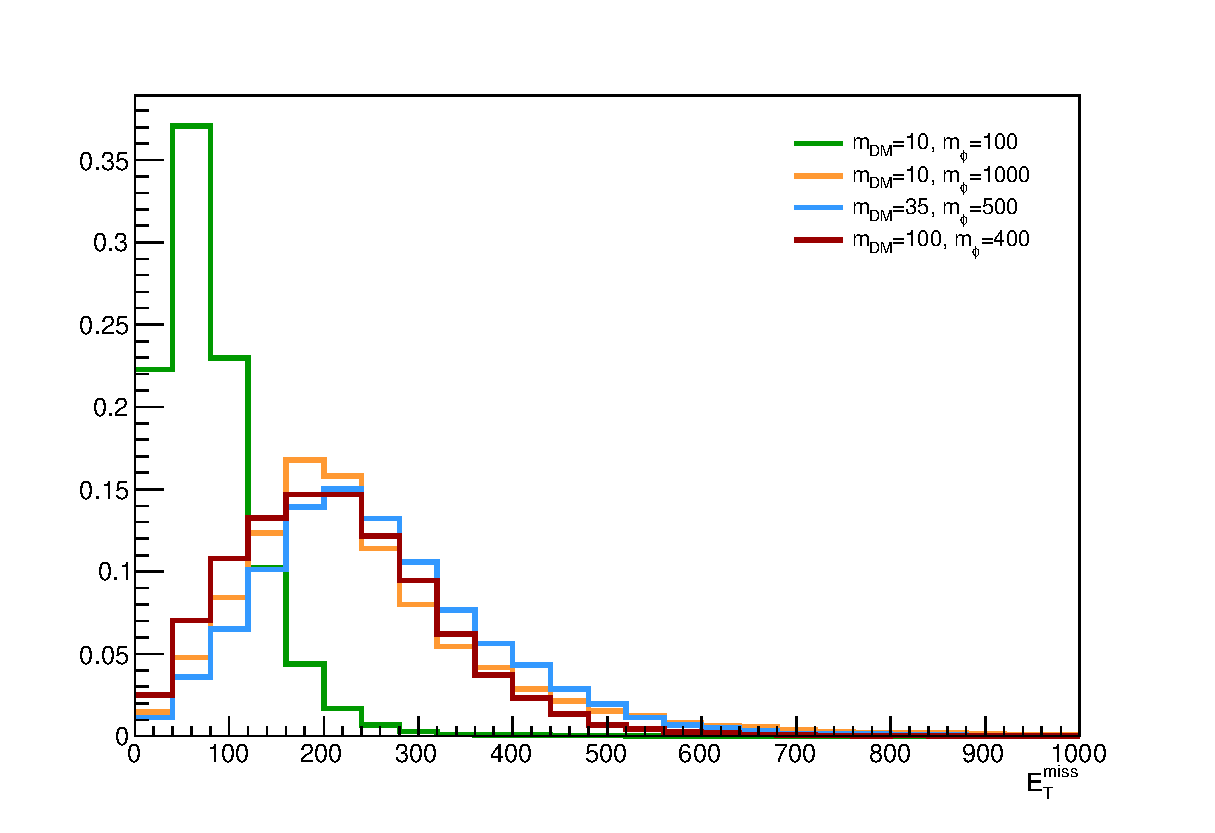
\includegraphics[scale=0.32]{figures/bFDM/bfdm_relic/missing_et.eps}
    \end{minipage}
    \hfill
    \begin{minipage}{0.49\textwidth}
      \centering 
      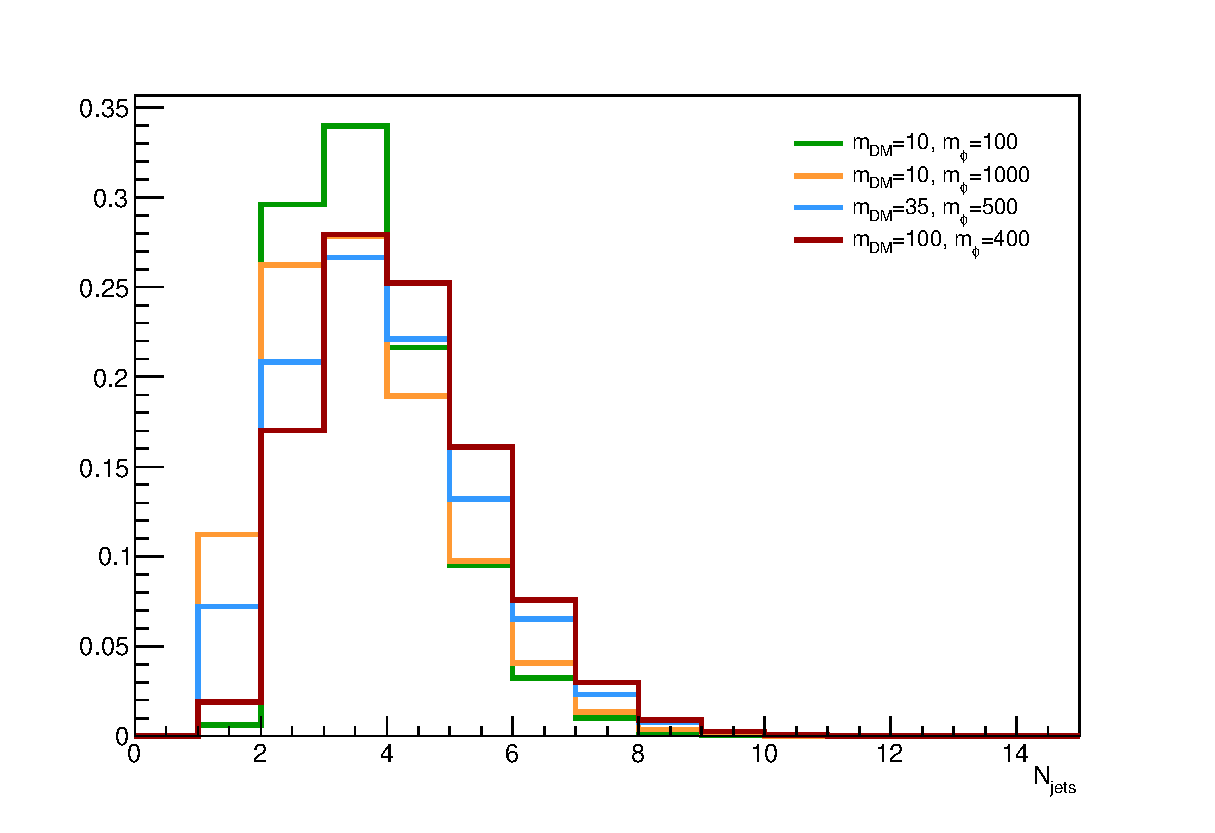
\includegraphics[scale=0.32]{figures/bFDM/bfdm_relic/Njets.eps}
    \end{minipage}
    \caption{MET (left) and jet multiplicity (right) for various DM and mediator masses and couplings normalised to the relic density observed in the early universe. \label{fig:relic}}
\end{figure}


\begin{figure}[h!]
    \begin{minipage}{0.49\textwidth}
      \centering 
      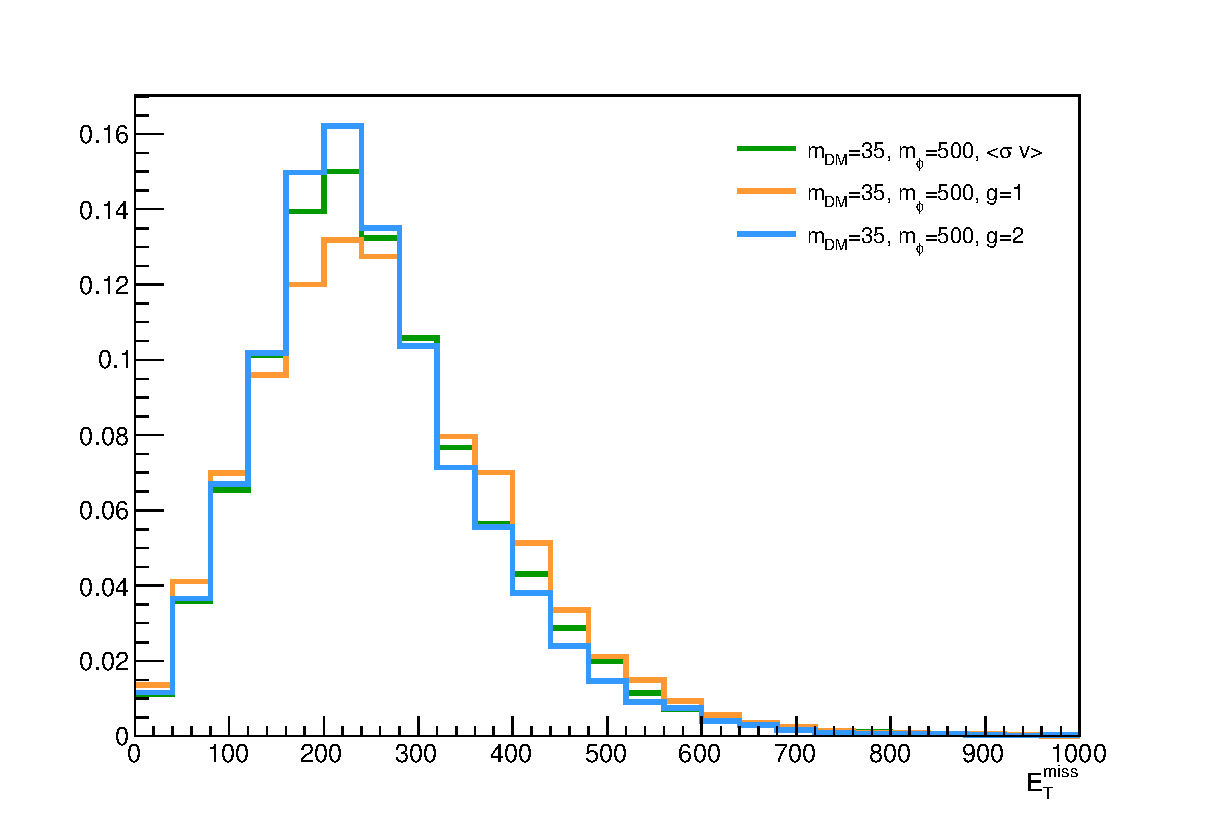
\includegraphics[scale=0.32]{figures/bFDM/bfdm_35_500/missing_et.eps}
    \end{minipage}
    \hfill
    \begin{minipage}{0.49\textwidth}
      \centering 
      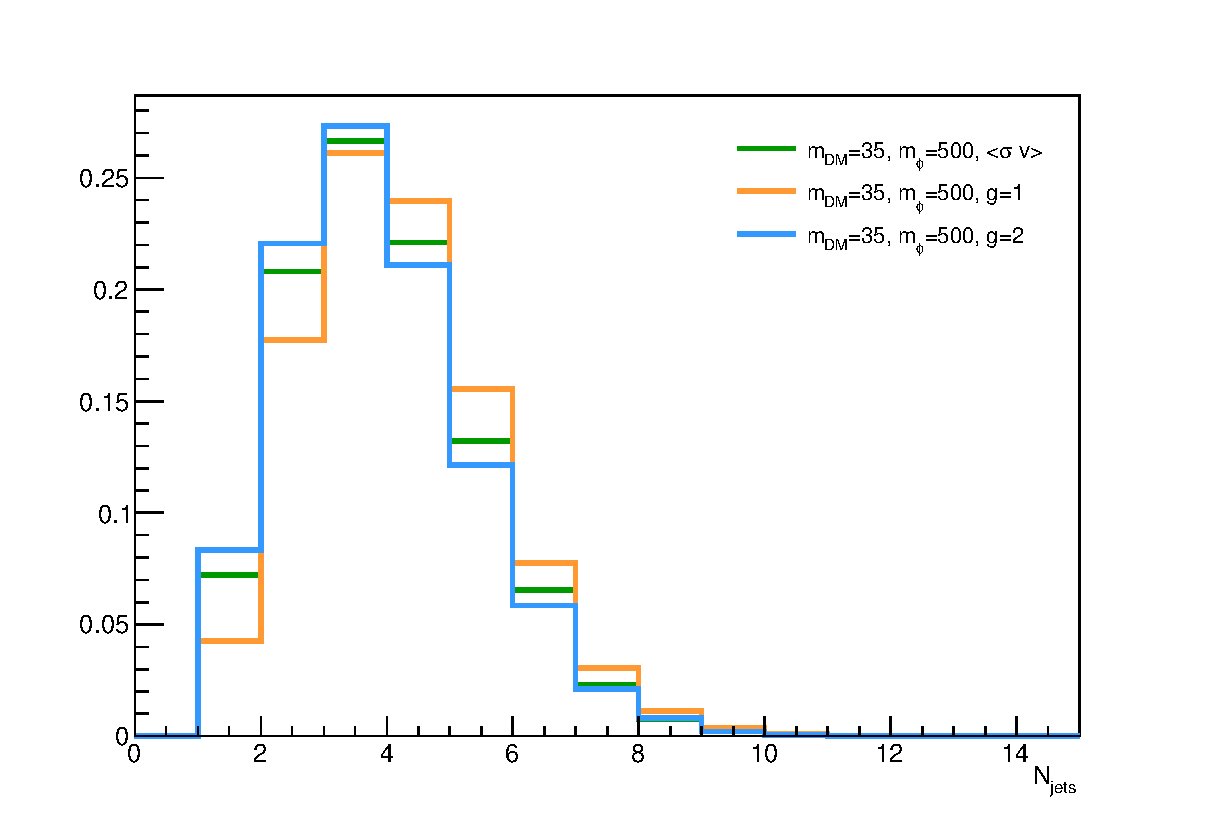
\includegraphics[scale=0.32]{figures/bFDM/bfdm_35_500/Njets.eps}
    \end{minipage}
    \caption{MET (left) and jet multiplicity (right) for $m_\textrm{DM}=35$~GeV and $m_\Phi=500$~GeV for couplings corresponding to relic density weights and also $g=1,2$ \label{fig:g_comp}}
\end{figure}

In light of these considerations, we recommend to produce the following benchmark points in the parameter space for this model:~\Todo{Describe the coupling scan?}

\begin{itemize}
  \item $m_\textrm{DM}=10-500$ GeV with a binning of 50 GeV for $m_\textrm{DM}<100$ and  100 GeV otherwise; 
  \item $m_\Phi=10-1300$ with a binning of 100 GeV;
  \item $m_\Phi > m_{DM} + m_b$, since the cross-sections in the off-shell region are too small to be sensitive with early LHC data;
\end{itemize}

Cross-sections for unit couplings can be found in Appendix~\ref{app:xsecs_bFDM}.
The increase in the center of mass energy from 8 to 13 TeV leads to a cross-section increase that is a function of $m_\Phi$, 
with a smaller dependency for $m_{\rm DM}$. Therefore, the sensitivity to this model will increase in early 
13~TeV data compared to 8 TeV searches~\cite{Aad:2014vea}.

\subsection{Model implementation}

\Todo{Do we have to match with Pythia PS? Do we have any recommendations for the initial state PDFs, given the heavy flavors?}

We simulate the model using the {\tt MG5\_aMC} v2.2.3. The corresponding card files can be found 
on the Forum SVN repository~\cite{ForumSVN_DMSingleB}.